\subsection{Solution of \eqref{eq:SI-StrongForm} via Finite-Differences} \label{ssec:SI-FDMMethod}
Now that we have the problem \eqref{eq:SI-StrongForm} to work with, we can attempt to solve \eqref{eq:SI-WaveEqn} through a formulation that involves familiar gradients and derivatives, rather than the more abstract tangential gradients.
Before we do so, it is convenient to notice that we can move the ``trace" terms in \eqref{eq:SI-InclusionEqn} to the left-hand-side to obtain the slightly nicer (in terms of the numerics that follow) looking system
\begin{subequations} \label{eq:SI-FDMEquationsToDisc}
	\begin{align}
		-\laplacian_\qm u 
		&= \omega^2 u 
		&\text{in } \ddom_i, \label{eq:SI-FDMBulk} \\
		- \bracs{\diff{}{y} + \rmi\qm_{jk}}^2u^{(jk)}  - \bracs{\bracs{\grad u\cdot n_{jk}}^+ - \bracs{\grad u\cdot n_{jk}}^-}
		&= \omega^2 u^{(jk)},
		&\text{in } I_{jk}, \label{eq:SI-FDMSkeleton} \\
		\sum_l \bracs{\pdiff{}{n}+\rmi\qm_{jk_l}} u^{(jk_l)}(v_j) 
		&= 0 
		&\text{at } v_j\in\vertSet. \label{eq:SI-FDMVertex}
	\end{align}
\end{subequations}
We have now placed everything except terms involving the spectral parameter on the left hand side of \eqref{eq:SI-FDMEquationsToDisc}, and our goal now is to devise a numerical scheme to approximate the action of the ``operators" on the left-hand-side, and from that approximate the spectrum of the problem.

Our idea is as follows; we recognise that $u$ is twice differentiable (in the familiar, classical sense) in each of the bulk regions and along each of the skeleton edges, so we can look to to approximate the spectrum of our problem by approximating $u$ through a (somewhat n{\"i}ave) finite-difference approximation in each of the bulk regions and skeleton edges, and tying these ``region-wise" approximations together.
To this end, we take each of the bulk regions $\ddom_i$, and place nodes $\tau_j\in\overline{\ddom}_{i}$ appropriately, so as to write finite difference approximations for $\laplacian_{\qm}u$ at each node $\tau_j\in\ddom_i$.
Note that, since $u$ is not required to be differentiable (in the classical sense) across the skeleton, it is important that any finite difference approximation at $\tau_j$ only uses the values of $u$ at other nodes in $\overline{\ddom}_{i}$.
In placing nodes in $\overline{\ddom}_{i}$, we will also end up with nodes placed on the portion of the skeleton (and vertices) that form part of $\partial\ddom_i$.
Since $u$ is twice differentiable along the skeleton, the placement of these nodes allows us to derive finite-difference approximations for the derivatives in \eqref{eq:SI-FDMSkeleton}.
The traces of the normal derivates (in \eqref{eq:SI-FDMSkeleton}) can also be approximated via one-sided differences using suitable nodes from each of the adjacent bulk regions.
Finally, an approximation for \eqref{eq:SI-FDMVertex} can be derived for nodes that lie at vertices $v_j\in\vertSet$, using the nodes that lie on edges that connect to $v_j$.
We will come to discuss some of the difficulties with the general application of this procedure after our illustrative example.
For now, let us assume we have approximations for the action of the gradient and derivative, so that the action of the left-hand-side of \eqref{eq:SI-FDMEquationsToDisc} is approximated through the action of a matrix $\mathcal{F}$ on the vector $U = \bracs{u_j}^\top$, where $u_j:=u\bracs{\tau_j}$.
We then approximate the system \eqref{eq:SI-FDMEquationsToDisc} by the matrix-eigenvalue problem involving $\mathcal{F}$.

Let us begin by illustrating this approach using the cross in the plane geometry.
We first discretise $\ddom$ into a uniform mesh consisting of $N\times N$ nodes $\tau_{p,q} = \bracs{(p-1)h,(q-1)h}$ for $p,q\in\clbracs{1,...,N}$, with a mesh width of $h = \recip{N-1}$, and write $u_{p,q} = u\bracs{\tau_{p,q}}$.
It is important to note at this early stage that we can utilise a uniform mesh thanks to the rather simple geometry of the skeleton, and in general the meshing process will be more complex (see the discussion at the end of this section).
Note that there is no need to place nodes along both of the periodic edges of $\ddom$, so long as we keep track of which nodes are connected by periodicity, but for notational purposes it is convenient to include such nodes in our description.
Proceeding with the discretisation of the above equations, $u$ is twice differentiable in the bulk region $\ddom^{\circ}$, and so at points $\tau_{p,q}\not\in\graph$ we can discretise as
\begin{align*}
	-\laplacian_\qm u\bracs{\tau_{p,q}} &\approx 
	\bracs{\abs{\qm}^2 + 4h^{-2}}u_{p,q}
	-h^{-1}\bracs{h^{-1} + \rmi\qm_1}u_{p+1,q}
	-h^{-1}\bracs{h^{-1} - \rmi\qm_1}u_{p-1,q} \\
	&\qquad -h^{-1}\bracs{h^{-1} + \rmi\qm_2}u_{p,q+1}
	-h^{-1}\bracs{h^{-1} - \rmi\qm_2}u_{p,q-1}, \labelthis\label{eq:SI-FDMBulkDiscretise}
\end{align*}
using centred differences.
One can also use forward (also known as left) or backward (a.k.a right) differences to approximate the $\laplacian_{\qm}$ operator --- this will likely be necessary for more complex skeleton geometries as was hinted at previously.
Also worth noting is that, should one choose not to use (or be unable to use) a uniform mesh, one will still obtain a similar expression to \eqref{eq:SI-FDMBulkDiscretise} for the approximation of $\laplacian_\qm u$ at a node $\tau\not\in\graph$, but in terms of the values of $u$ at, and the distances to, the ``nearest neighbour" nodes to $\tau$.

For nodes $\tau_{p,q}\in I_{jk}$ (for either $I_{jk}=I_h$ or $I_v$), our finite difference approximations become slightly more complex as we are forced to consider the nearest nodes to $\tau_{p,q}$ that lie in the directions $e_{jk}$ and $n_{jk}$.
This is because $u$ is twice differentiable \emph{along the skeleton}, so we must approximate $\bracs{\diff{}{y} + \rmi\qm_{jk}}^2u^{(jk)}$ through finite differences along the edge $I_{jk}$, which will involve the values of $u$ at the nodes ``adjacent" to $\tau_{p,q}$ in the $e_{jk}$ and $-e_{jk}$ directions.
For the normal-derivative trace terms, we use one-sided finite differences to approximate these values at $\tau_{p,q}$, which involves the values of $u$ at the nodes ``adjacent" to $\tau_{p,q}$ in the $n_{jk}$ and $-n_{jk}$ directions.
For general skeleton geometries these requirements will contribute to the complications with meshing the domain, but since the edges are aligned with the coordinate axes in the cross-in-the-plane geometry, the vectors $e_{jk}$ and $n_{jk}$ are also aligned with the coordinate axes and the discretisation proceeds easily.
Those $\tau_{p,q}$ that lie on the horizontal edge $I_h$ have $q=0$ and $p\neq0$, so our finite difference approximation is
\begin{align*}
	- & \bracs{\diff{}{y} + \rmi\qm_{jk}}^2 u_{p,0} - \bracs{\bracs{\grad u_{p,0}\cdot n_{jk}}^+ - \bracs{\grad u_{p,0}\cdot n_{jk}}^-} \\
	& \quad\approx \bracs{\qm_1^2 + 2h^{-1} + 2h^{-2}}u_{p,0}
	- h^{-1}\bracs{h^{-1} + \rmi\qm_1}u_{p+1,0}
	- h^{-1}\bracs{h^{-1} - \rmi\qm_1}u_{p-1,0} \\
	& \quad - h^{-1}u_{p,1} - h^{-1}u_{p,-1}. \labelthis\label{eq:SI-FDMHorzEdgeDiscretise}
\end{align*}
Here we have used centred differences along the edge $I_h$, identifying that the nodes $\tau_{p-1,0}, \tau_{p+1,0}$ are the adjacent nodes in the $x_1 (= e_h)$ direction.
The traces cause the introduction of the terms $u_{p,-1}$ and $u_{p,1}$, since $-x_2 = n_h$.
Analogously, nodes $\tau_{p,q}$ on the vertical edge $I_v$ have $p=0$ and $q\neq0$, and the finite difference approximation is
\begin{align*}
	- & \bracs{\diff{}{y} + \rmi\qm_{jk}}^2 u_{0,q} - \bracs{\bracs{\grad u_{0,q}\cdot n_{jk}}^+ - \bracs{\grad u_{0,q}\cdot n_{jk}}^-} \\
	& \quad\approx \bracs{\qm_2^2 + 2h^{-1} + 2h^{-2}}u_{0,q}
	- h^{-1}\bracs{h^{-1} + \rmi\qm_2}u_{0,q+1}
	- h^{-1}\bracs{h^{-1} - \rmi\qm_2}u_{0,q-1} \\
	& \quad - h^{-1}u_{1,q} - h^{-1}u_{-1,q}. \labelthis\label{eq:SI-FDMVertEdgeDiscretise}
\end{align*}

Finally, we come to the node $\tau_{0,0}$ placed at the vertex $v_0$.
Our finite difference approximation already enforces that $u$ be continuous at $v_0$, so we just have to enforce the vertex condition at this node.
Here we again approximate each (signed) normal derivative by a one-sided finite difference from the adjacent edges, giving us
\begin{align} \label{eq:SI-FDMVertCond}
	\sum_{j\con k}\bracs{ \pdiff{}{n} + \rmi\qm_{jk} }u_{0,0}
	&\approx h^{-1} \bracs{ 4u_{0,0} - u_{1,0} - u_{-1,0} - u_{0,1} - u_{0,-1} }.
\end{align}
We now insert these finite difference approximations \eqref{eq:SI-FDMBulkDiscretise}-\eqref{eq:SI-FDMVertCond} into \eqref{eq:SI-FDMEquationsToDisc}, which provides the following system in the $\bracs{N-1}^2$ nodal values $u_{p,q}$;
\begin{subequations} \label{eq:SI-FDMDiscreteEqns}
	\begin{align*}
		\bracs{\abs{\qm}^2 + 4h^{-2}} & u_{p,q}
		-h^{-1}\bracs{h^{-1} + \rmi\qm_1}u_{p+1,q}
		-h^{-1}\bracs{h^{-1} - \rmi\qm_1}u_{p-1,q} \\
		& -h^{-1}\bracs{h^{-1} + \rmi\qm_2}u_{p,q+1}
		-h^{-1}\bracs{h^{-1} - \rmi\qm_2}u_{p,q-1}
		= \omega^2 u_{p,q}, & p,q\neq0, \labelthis\label{eq:SI-FDMBulkDiscEqns} \\
		\bracs{\qm_1^2 + 2h^{-1} + 2h^{-2}} & u_{p,0}
		-h^{-1}\bracs{h^{-1} + \rmi\qm_1}u_{p+1,0}
		-h^{-1}\bracs{h^{-1} - \rmi\qm_1}u_{p-1,0} \\
		& -h^{-1}u_{p,1} - h^{-1}u_{p,-1}
		= \omega^2 u_{p,0}, & p\neq0, q=0, \labelthis\label{eq:SI-FDMHEdge} \\
		\bracs{\qm_2^2 + 2h^{-1} + 2h^{-2}} & u_{0,q}
		-h^{-1}\bracs{h^{-1} + \rmi\qm_2}u_{0,q+1}
		-h^{-1}\bracs{h^{-1} - \rmi\qm_2}u_{0,q-1} \\
		& -h^{-1}u_{1,q} - h^{-1}u_{-1,q}
		= \omega^2 u_{0,q}, & p=0, q\neq0, \labelthis\label{eq:SI-FDMVEdge} \\
		h^{-1} & \bracs{ 4u_{0,0} - u_{1,0} - u_{-1,0} - u_{0,1} - u_{0,-1} }
		= 0, & p=q=0, \labelthis\label{eq:SI-FDMDiscVertex}
	\end{align*}
\end{subequations}
where $p,q\in\clbracs{0,...,N-1}$ unless otherwise stated.
This system can then be written in matrix form as 
\begin{align} \label{eq:SI-FDMMatrixEqn}
	\mathcal{F}U &= \omega^2 B U,
\end{align}
where $B=\mathrm{diag}\bracs{1,...,1,0,1,...,1}$ is a (positive semi-definite) diagonal matrix with the zero in the row corresponding to the equation \eqref{eq:SI-FDMDiscVertex}.
The equation \eqref{eq:SI-FDMMatrixEqn} can then be solved using a generalised eigenvalue solver to obtain the approximate eigenvalues $\omega^2$ and eigenvectors $U$.

The approximate eigenvalues computed by the finite difference scheme using $N=251$ grid-points in each of the coordinate directions are displayed in figure \ref{fig:CompositeCross-FDM-SpectralBands}.
\begin{figure}[b!]
	\centering
	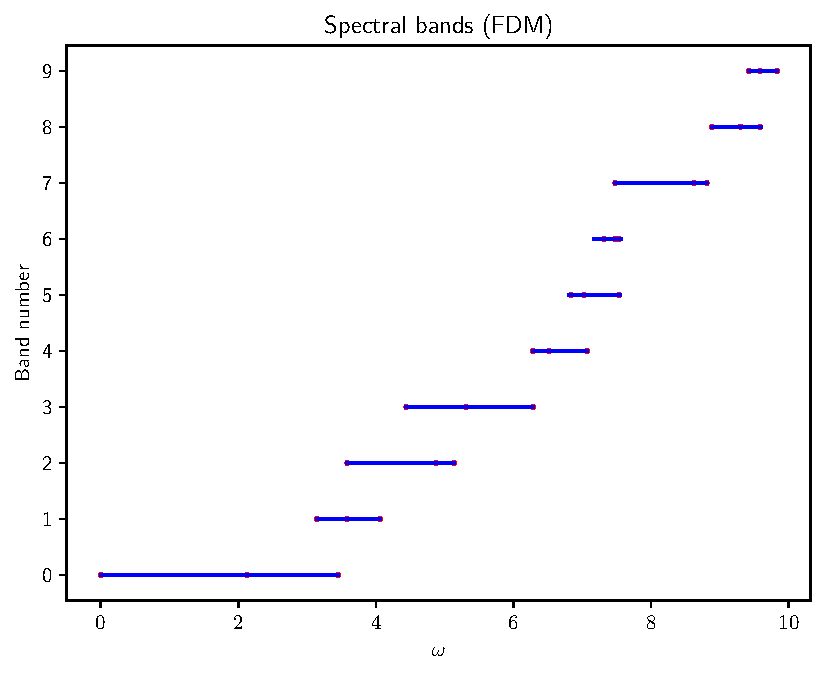
\includegraphics[scale=0.5]{CompositeCross-FDM-SpectralBands.pdf}
	\caption{\label{fig:CompositeCross-FDM-SpectralBands} The approximate eigenvalues computed by the finite-difference scheme, sorted into spectral bands for the cross-in-the-plane geometry. Eigenvalues corresponding to the extremities of the quasi-momentum are plotted in red.}
\end{figure}
Those points plotted in red correspond to eigenvalues that were computed at quasi-momentum values of $\bracs{0,0}^\top$, $\bracs{-\pi,0}^\top$, $\bracs{0,-\pi}^\top$, $\bracs{-\pi,-\pi}^\top$, from which we can observe that these points typically form the endpoints of each of the spectral bands.
Much like the quantum graph case, we do not expect this to occur for general geometries --- there even appears to be a notable example of this in band 6, for which the eigenvalues at the extremities of the band are not obtained at any of these quasi-momentum values.
However by examining the eigenvalues in this band as functions of $\qm$, as in figure \ref{fig:FDM_2022-01-28-09-33_AllBands}, it can be noticed that these extreme eigenvalues occur at quasi-momentum values where one of the components is either 0 (for the minimum values) or $-\pi$ (for the maximum values).
\begin{figure}[b!]
	\centering
	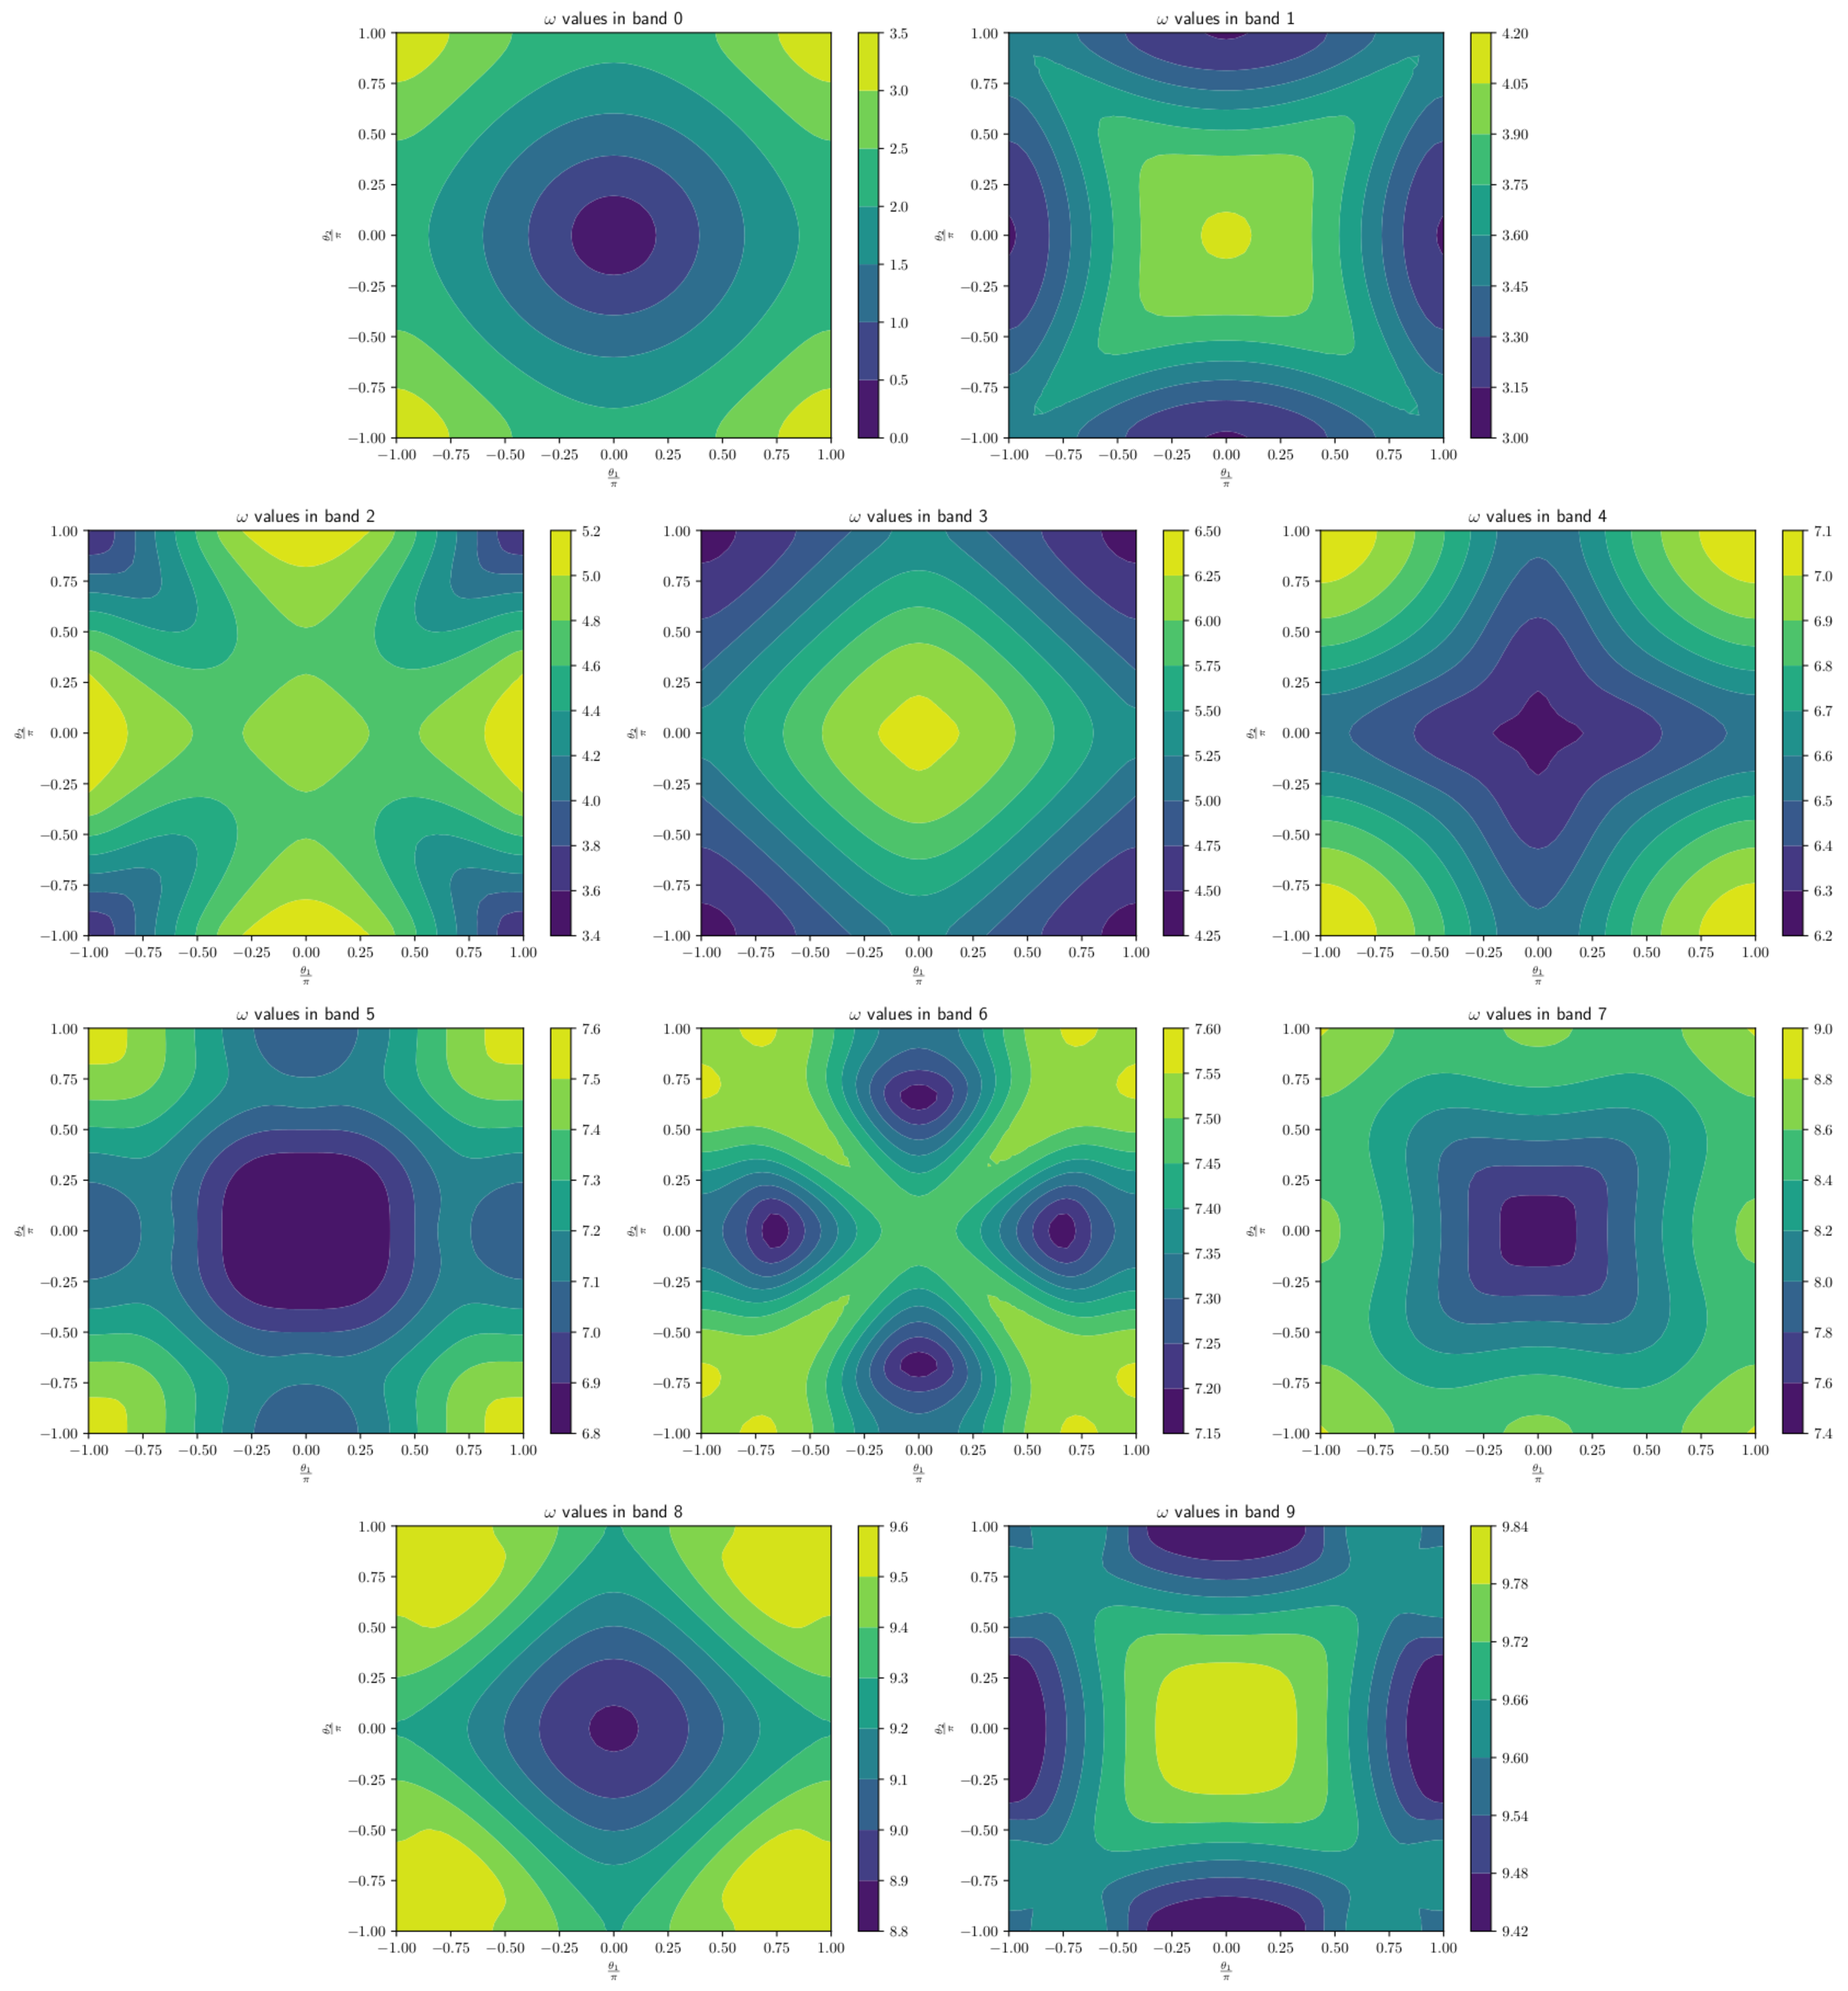
\includegraphics[width=\textwidth]{FDM_2022-01-28-09-33_AllBands.pdf}
	\caption{\label{fig:FDM_2022-01-28-09-33_AllBands} The eigenvalues $\omega$ in each spectral band, plotted as functions of the quasi-momentum $\qm$. Observe the symmetries that are expected from proposition \ref{prop:CrossInPlaneSymmetries}.}
\end{figure}
Similarly to our approach via \eqref{eq:SI-VarProb}, the eigenvalues within each band obey the symmetries expected from proposition \ref{prop:CrossInPlaneSymmetries}.

A distinct advantage of using this method over that for solving problem \ref{prob:DiscVarProb} is that, once the finite difference matrix $\mathcal{F}$ is assembled, we can use matrix-eigenvalue solvers to examine the eigenvalues near to any positive number that we choose, without needing to compute \emph{all} the previous eigenvalues (and eigenfunctions) up to this value.
This allows us to easily test the rate of convergence of the numerical scheme to the eigenvalues $\omega_{n,m}^2 = \bracs{n^2+m^2}\pi^2$.
In these cases, we expect that the error in the approximate eigenvalue is of the order of $N^{-2}$, since our scheme makes use of centred differences in the bulk region, and on the skeleton the eigenfunction should be identically zero.
This is what we observe numerically, and is illustrated in figure \ref{fig:CompositeCross-FDM-DEV} for $n\leq m\in\clbracs{1,2,3}$ (the cases $n>m$ are similar due to the aforementioned symmetry).
\begin{figure}[h]
	\centering
	\begin{subfigure}[t]{0.45\textwidth}
		\centering
		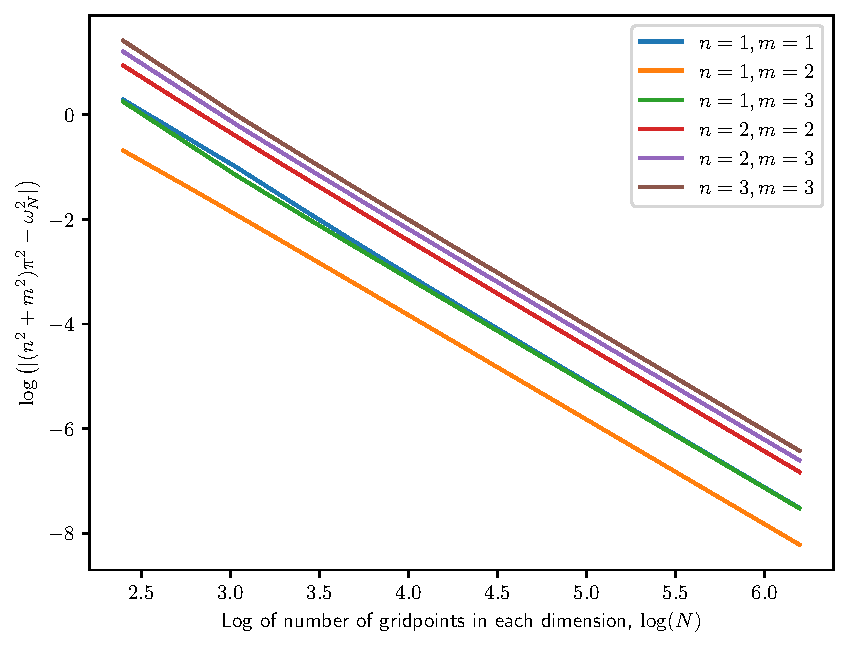
\includegraphics[scale=0.45]{CompositeCross-FDM-DEV-LogError.pdf}
		\caption{\label{fig:CompositeCross-FDM-DEV-LogError} Logarithm of the error in the eigenvalue against $\log(N)$, for a selection of $n,m$ values.}
	\end{subfigure}
	~
	\begin{subfigure}[t]{0.45\textwidth}
		\centering
		\begin{tabular}[b]{| c | c | c |}
			\hline
			$\bracs{n,m}$ & Intercept & Gradient \\
			\hline
			$\bracs{1, 1}$ & $5.14236963$ & $-2.04617746$ \\
			\hline
			$\bracs{1, 2}$ & $4.14218510$ & $-1.99442370$ \\
			\hline
			$\bracs{1, 3}$ & $4.96573274$ & $-2.01780686$ \\
			\hline
			$\bracs{2, 2}$ & $5.70851785$ & $-2.02509086$ \\
			\hline
			$\bracs{2, 3}$ & $5.95893392$ & $-2.03031478$ \\
			\hline
			$\bracs{3, 3}$ & $6.14879571$ & $-2.03187802$ \\
			\hline
		\end{tabular}
		\caption{\label{fig:CompositeCross-FDM-DEV-LoBF} Line of best fit (via least squares regression) for each pair $\bracs{n,m}$.}
	\end{subfigure}
	\caption{\label{fig:CompositeCross-FDM-DEV} Convergence rate for the FDM method to the analytic eigenvalues shared with the Dirichlet laplacian. Observe that the estimated gradient, hence convergence rate with $N$, is approximately $-2$ as expected.}
\end{figure}
Regrettably, we do not have to hand any analytic solutions to \eqref{eq:SI-WaveEqn} beyond those shared with the Dirichlet laplacian and so we cannot test the rate of convergence for solutions which are non-constant along the skeleton. \tstk{but we could include some pictures of them anyway, right?}

Our example using the cross-in-the-plane geometry illustrates the principle behind this approach; use finite differences to approximate $u$ in each $\ddom_i$ and along each $I_{jk}$, and tie approximations from adjacent bulk regions together through the nodal values along the common edge of the skeleton.
Compared to the variational approach in section \ref{sec:SI-VarProbMethod}, this approach avoids working with $\compMes$ directly and instead allows us to work solely in terms of classical derivatives, approximating them through Taylor's theorem.
However by choosing to approximate our function within each region and then ``stitch" these approximations together, we must choose our mesh in such a way as to abide by this decision, which can lead to some further considerations.
Let us begin by considering the requirements of the placement of nodes within the bulk regions --- each node must have neighbours in each of the coordinate directions that lie within the (closure of) the bulk region.
Now, consider a bulk region like that in figure \ref{fig:Diagram_FDMMeshIssue}, where a part of the skeleton is not aligned to the coordinate axes.
\begin{figure}[t]
	\centering
	\begin{subfigure}[t]{0.3\textwidth}
		\centering
		\includegraphics[scale=1.0]{Diagram_FDMMeshIssue-a.pdf}
		\caption{\label{fig:Diagram_FDMMeshIssue-a} A uniform mesh does not ensure that nodes in the bulk regions have neighbouring nodes which will provide us with a $C^2$-approximation, nor that every vertex has a node placed at it.}
	\end{subfigure}
	~
	\begin{subfigure}[t]{0.3\textwidth}
		\centering
		\includegraphics[scale=1.0]{Diagram_FDMMeshIssue-b.pdf}
		\caption{\label{fig:Diagram_FDMMeshIssue-b} Placing additional nodes along the skeleton edges, ensuring nodes in the bulk region have neighbours that lie within that same bulk region or on its boundary.}
	\end{subfigure}
	~
	\begin{subfigure}[t]{0.3\textwidth}
		\centering
		\includegraphics[scale=1.0]{Diagram_FDMMeshIssue-c.pdf}
		\caption{\label{fig:Diagram_FDMMeshIssue-c} The nearest nodes in the directions $\pm n_{jk}$ from the skeleton may be far from the edge or not exist at all (left highlighted node). Interpolation (right highlighted node) offers a solution, provided the bulk region is meshed well.}
	\end{subfigure}
	\caption{\label{fig:Diagram_FDMMeshIssue} An illustration of the complications encountered and considerations to be made when setting up a finite difference based approach for a general skeleton.}
\end{figure}
As we can quickly realise, uniform mesh will not be sufficient in this case, nor in general when the skeleton has edges that are not aligned to the coordinate axes. 
In figure \ref{fig:Diagram_FDMMeshIssue-a}, the highlighted node in the bulk region has no neighbour ``below" that lies within the same bulk region or its boundary, so a centred difference approximation to $\laplacian_{\qm}u$ at this node cannot be used.
One could argue that a suitable value for $u$ ``below" the highlighted node could be read off from interpolating values between nodes along the edge (then applying the knowledge that $u$ is continuous across the skeleton).
However there is no assurance that this interpolation will produce an accurate value for $u$, particularly if we are in the situation in figure \ref{fig:Diagram_FDMMeshIssue-a} where there are only two nodes along the diagonal edge, and the lower-left vertex doesn't even have a node placed at it.
To address this meshing complication, one can introduce additional nodes along the skeleton (and at the vertices) where necessary, as in figure \ref{fig:Diagram_FDMMeshIssue-b} (highlighted in blue).
This results in every node in the bulk regions having suitable neighbours in the coordinate directions, and has the additional bonus of improving the approximation of the derivative of $u$ along the skeleton.
Our expense is that we have given up a uniform distance between all nodes, which will require us to take slightly care when deriving difference equations at each node and assembling the matrix $\mathcal{F}$, and the rate of convergence will likely scale with some power of the \emph{greatest} such inter-nodal distance.

We also may end up compounding another issue when we come to approximate the normal derivative traces in \eqref{eq:SI-FDMSkeleton}, which we highlight in figure \ref{fig:Diagram_FDMMeshIssue-c} --- if an edge is not aligned with the coordinate axes, where are the nearest nodes in the directions $\pm n_{jk}$ from the edge?
There is the possibility that such a node is far from the edge, again resulting in a poor approximation to the trace of the normal derivative, or that such a node may not even exist (see the leftmost highlighted node in figure \ref{fig:Diagram_FDMMeshIssue-c}).
We again have the option of interpolating a value for $u$ in the bulk regions, schematically illustrated at the right highlighted node in figure \ref{fig:Diagram_FDMMeshIssue-c} --- the values at the orange points can be interpolated from nodes in the bulk region, provided we have already made sensible mesh choices within the adjacent bulk regions\footnote{Note that we cannot simply decide to make the mesh in the bulk region finer, so that a node is placed in the position we want to interpolate. In general, doing so will end up in us requiring more nodes on the skeleton through the issue in figure \ref{fig:Diagram_FDMMeshIssue-a}, sending us in circles!}.
These issues arise due to how the skeleton (or more precisely, each edge of the skeleton) is effectively using a different coordinate system (for its derivatives) to the bulk regions, which is why this issue disappears when the edges of the skeleton are aligned to the coordinate axes --- the ``neighbouring" nodes we need on the skeleton are in the directions $e_{jk}, n_{jk}$ rather than the coordinate directions $x_1, x_2$.
Whilst the complications this brings can be combatted in the manners discussed above, it does highlight the need for care when setting up and implementing this approach for general skeleton geometries.
Contrastingly, the approach via \eqref{eq:SI-VarProb} does not run into these issues since (in that approach) we have made the choice to work with $\compMes$ directly and approximate the related gradients globally (over the whole domain) rather than utilising their properties on sub-regions.

\tstk{could have a final paragraph or two commenting on a finite element based approach, which is a middle ground between the two approaches discussed here. It uses the variational form, but the basis functions that we'll be using would be local... Move to discussion at end}